\documentclass[16pt]{beamer}
\usetheme{Berkeley}
\usepackage[utf8]{inputenc}
\usepackage[english]{babel}
\usepackage{amsmath}
\usepackage{amsfonts}
\usepackage{amssymb}
\usepackage{graphicx}
\author{Stefan Zaufl, Dominik Schörkhuber}
\title{High-Quality Surface Splatting on Today's GPUs}
%\setbeamercovered{transparent} 
%\setbeamertemplate{navigation symbols}{} 
%\logo{} 
%\institute{} 
%\date{} 
%\subject{} 
\begin{document}

\begin{frame}
\titlepage
\end{frame}

%\begin{frame}
%\tableofcontents
%\end{frame}

\begin{frame}{Splatting}
\begin{figure}[hbtp]
\centering
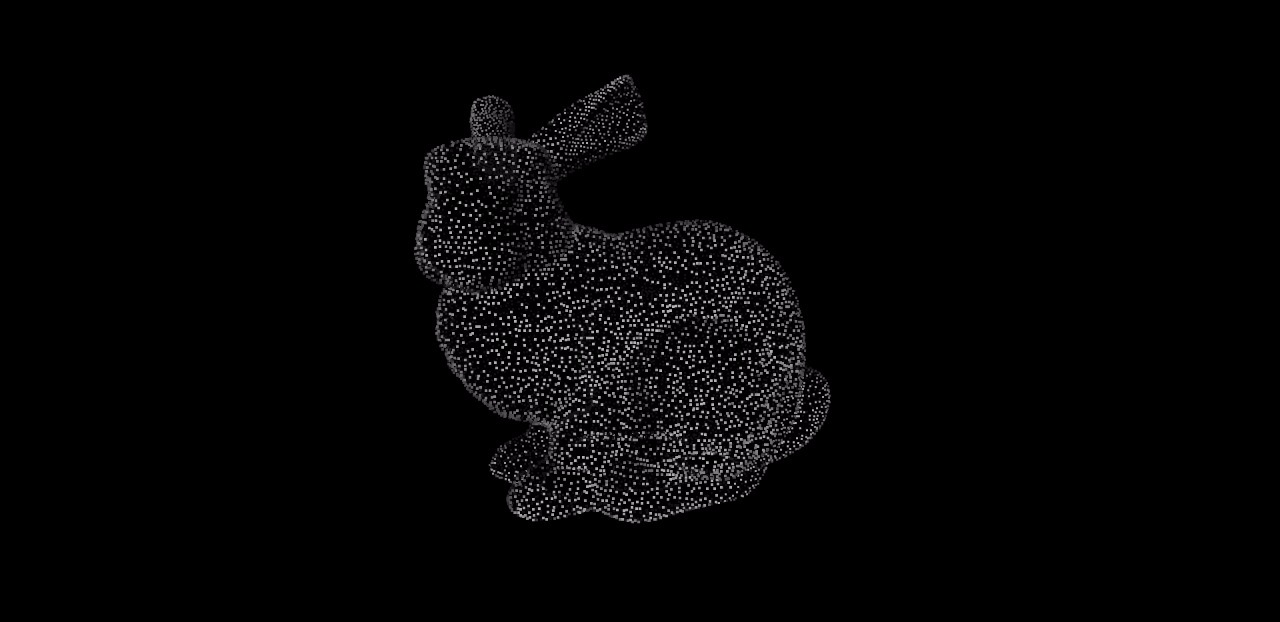
\includegraphics[width=\textwidth]{img/bunny_small}
\end{figure}
\end{frame}

\begin{frame}{Compute the Splat Attributes}
\begin{figure}[hbtp]
\centering
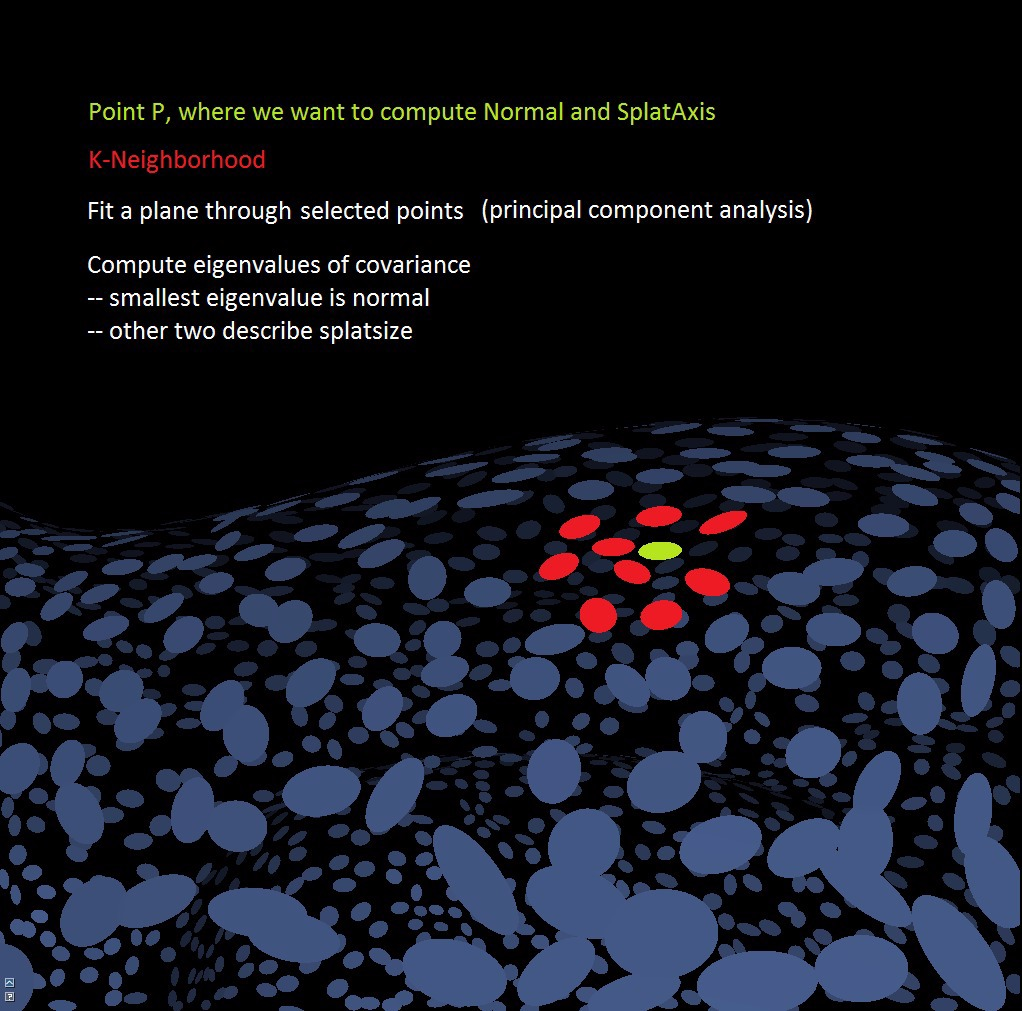
\includegraphics[width=\textwidth]{img/splat_neighbours}
\end{figure}
\end{frame}

\begin{frame}{Splatting}
\begin{figure}[hbtp]
\centering
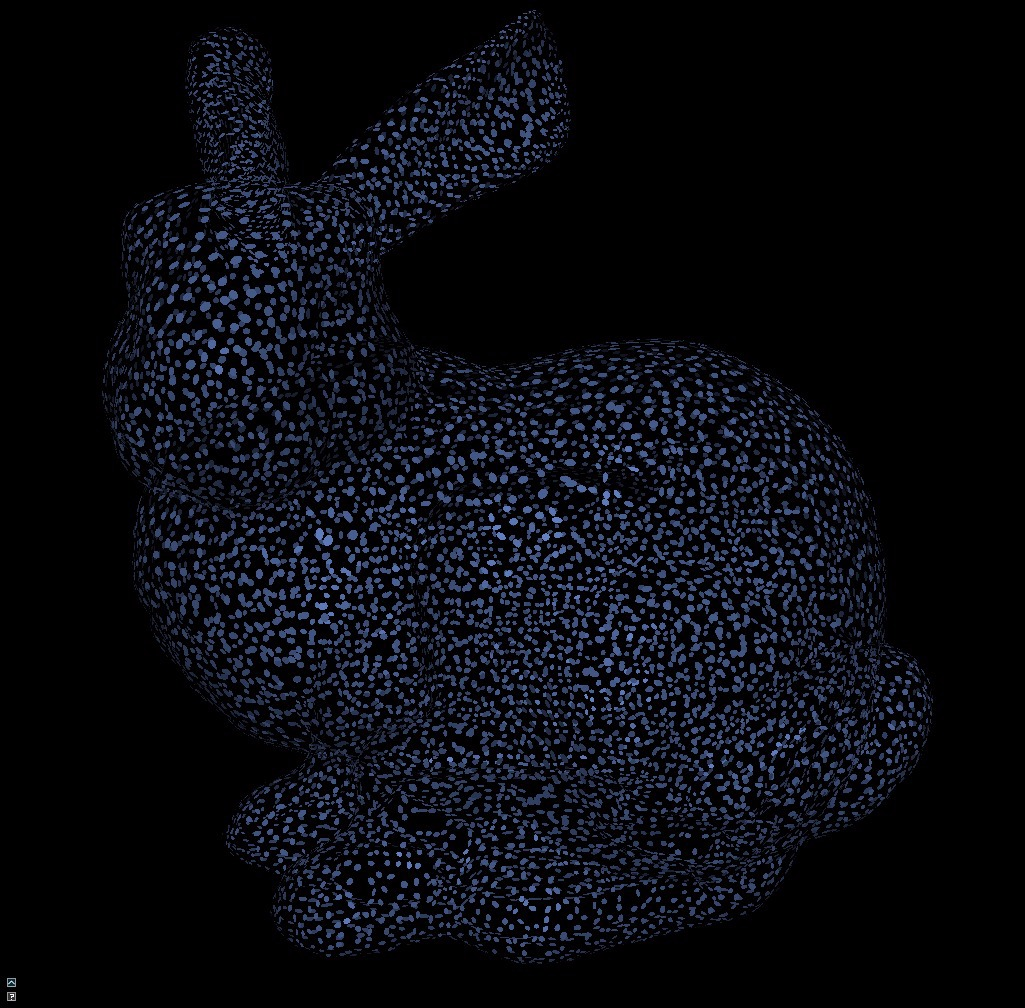
\includegraphics[width=\textwidth]{img/bunny_holes}
\end{figure}

\end{frame}

\begin{frame}{Splatting}
\begin{figure}[hbtp]
\centering
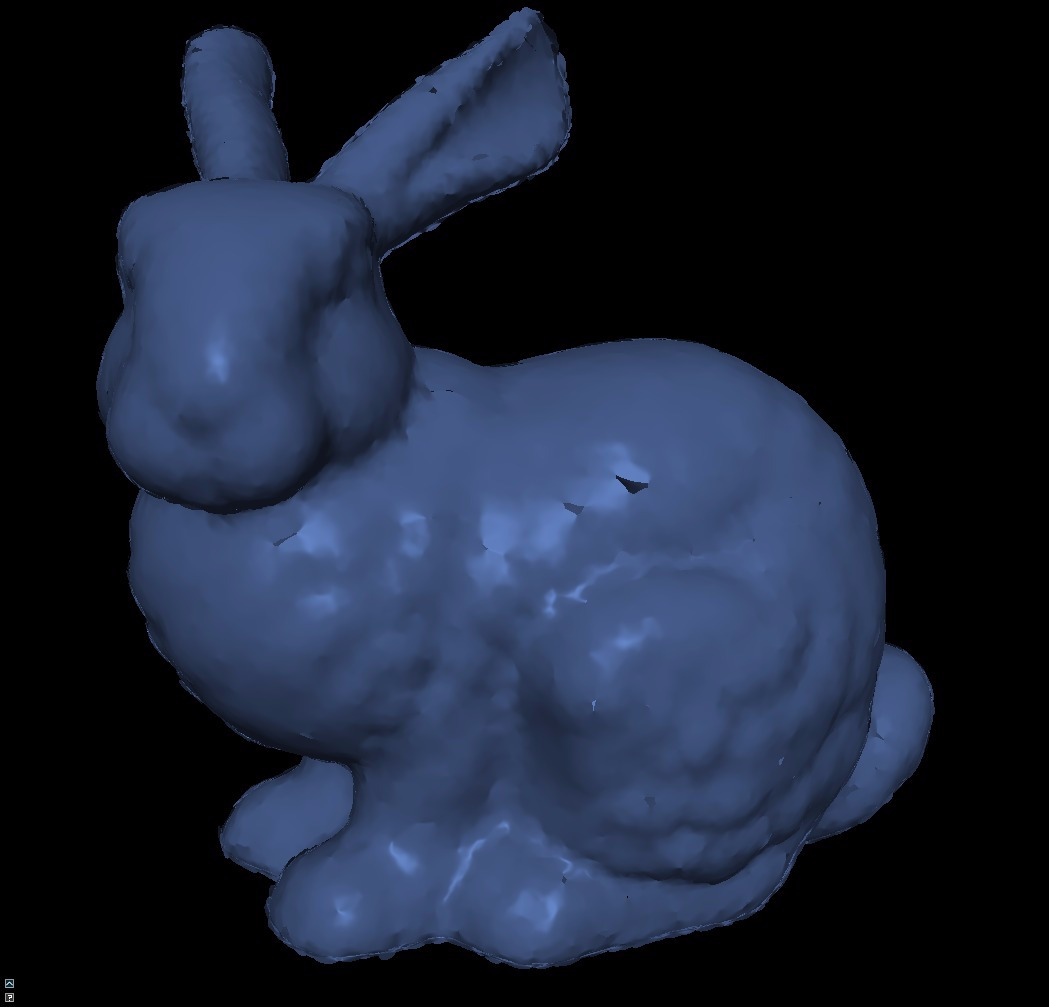
\includegraphics[width=\textwidth]{img/bunny_big}
\end{figure}

\end{frame}

\begin{frame}{Deferred Rendering Pipeline}
\begin{figure}[hbtp]
\centering
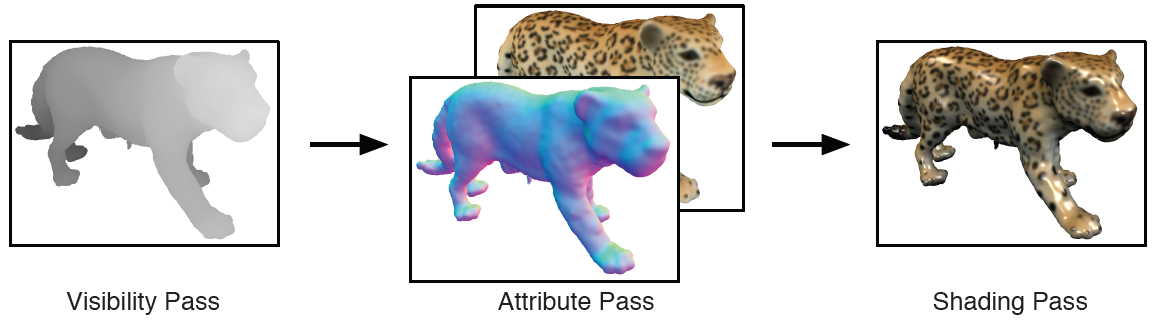
\includegraphics[width=\textwidth]{img/Passes}
\end{figure}


\begin{enumerate}
\item Identify visible points
\item Accumulate attributes
\item Normalization and shading
\end{enumerate}

\end{frame}

\begin{frame}{EWA Filtering}
\begin{figure}[hbtp]
\centering
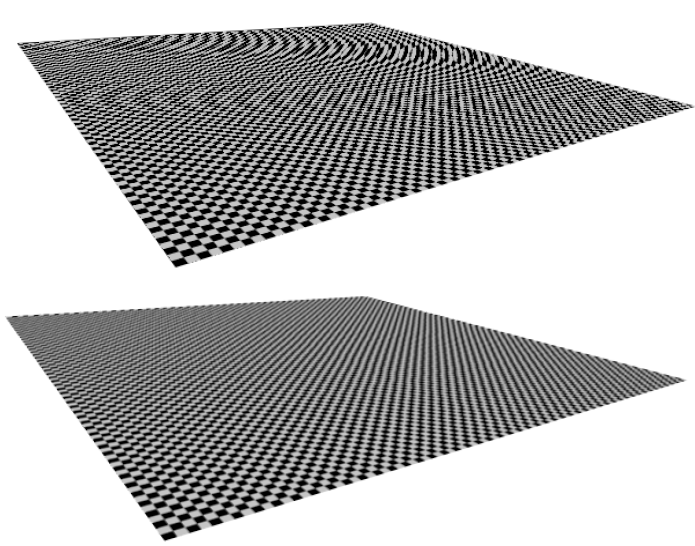
\includegraphics[width=\textwidth]{img/EWA_filter}
\end{figure}

\end{frame}

\end{document}